\svnid{$Id: rt_overview.tex 1 2015-10-01 14:54:12Z rodriqu_dd $}

\chapter{General overview of the GUI}
\label{chap:rt_overview}

This chapter introduces all GUI-components, which are shared between applications based on the framework.
%
\section{Windows}
\label{sec:windows}
As DeltaShell is an integrated modelling suite, the application is project-based. Within a project several models may be run and combined.

The main user interface is organized in a set of tool and document windows. An example is given in \Fref{fig:fig3.1}. The tool windows show properties of the current project, whereas document windows are used to visualize or edit a specific data type. Tool windows can be docked where you prefer --- even at a second display. Document windows are, when placed within the framework, always in the central area but may also be docked stand-alone (on a second display, for example). Examples of tool windows are:
%
\begin{itemize}
	\item \window{Project}
	\item \window{Map}
	\item \window{Properties}
	\item \window{Chart}
	\item \window{Messages}
\end{itemize}
%
Examples of document windows are:
%
\begin{itemize}
	\item Map(s)
	\item Editor(s)
\end{itemize}
%
\begin{figure} [H]
	\centering
		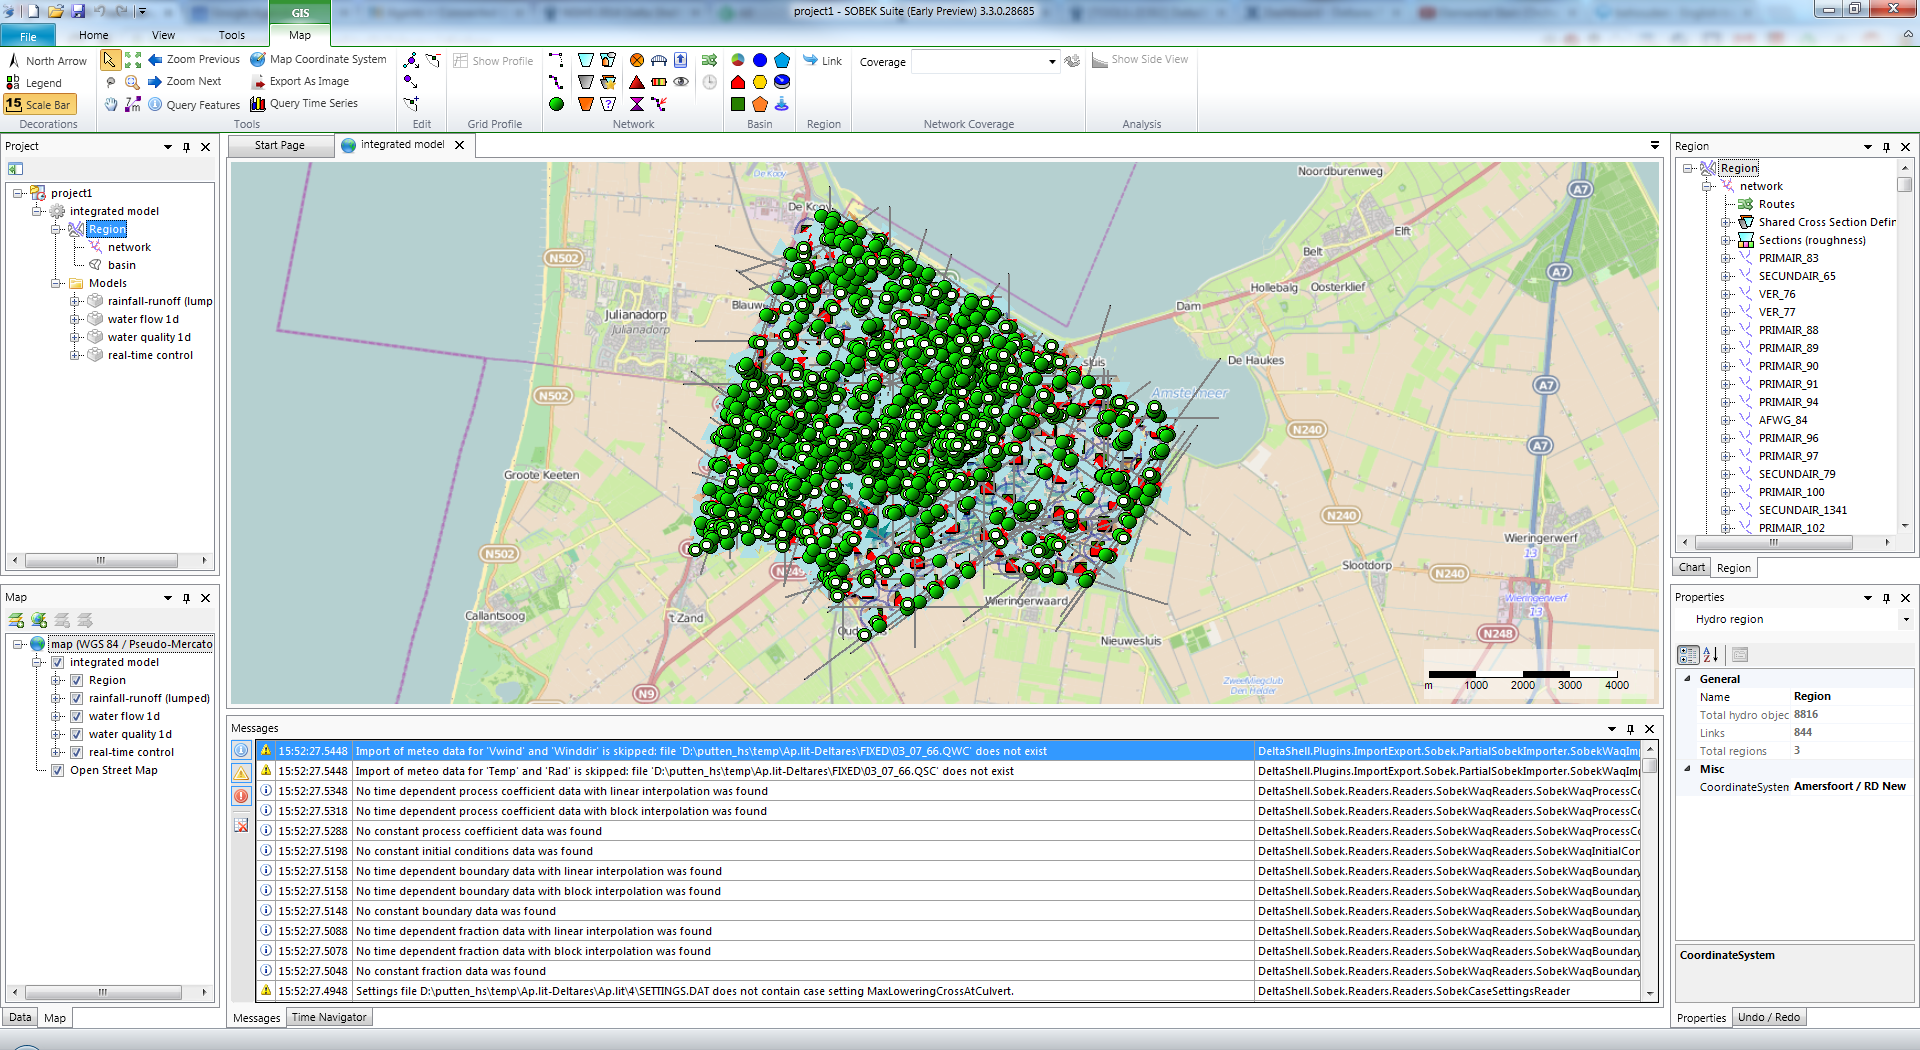
\includegraphics[width=\textwidth]{figures/chapter_overview/overview_ds}
	\caption{Overview of the graphical user interface, example for a SOBEK3 model.}
	\label{fig:fig3.1}
\end{figure}
%
In this chapter all tool windows, menus, dockable views, context menus, and ribbons and toolbars will be described. Map functionality and the spatial editor are treated in separate chapters. The specific editors for the different models are described in the user manuals belonging to those model plug-ins.

\subsection{Project}
\label{subsec:project}
The \window{Project} window is the main navigation window for the project data, showing the total workspace in a tree view (\Fref{fig:figoverview.2}). In the \window{Project} all project components are shown. 
%
All project items with sub-levels can be collapsed by a mouse-click on the `$-$' sign in the tree view. Project data can be sorted by adding new folders to the project tree view and moving models or movable items to designated folders.
%
By clicking on the top left icon in \Fref{fig:figoverview.2} the active item in the central Map is located in the tree view.
%
\begin{figure} [H]
	\centering
		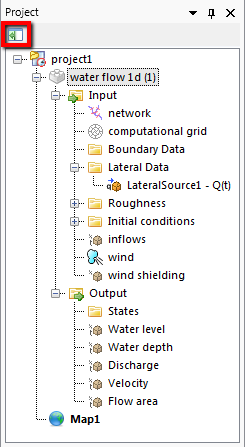
\includegraphics[width=0.5\textwidth]{figures/chapter_overview/view_project_window.png}
	\caption{The project tree window.}
	\label{fig:figoverview.2}
\end{figure}
%
Several possibilities exist to work with the tree view:
%
\begin{itemize}
	\item Left mouse-click to select
	\item Right mouse-click gives a context menu with available actions
	\item Double-click to show a map or editor in the main (central) window, depending on the parameter
\end{itemize}
%
\subsection{Main (central) window}
\label{subsec:Main}
The main window (\Fref{fig:fig2.3}) is by default always placed in the middle of the screen. It can also be docked separately, for example on a second display. It is used to present a map for all geo-referenced modeldata, the editors for other data, and results in charts. The editors for other data are model-specific and therefore described in the manuals for the various model plug-ins.

All items with a geo-reference will be presented on the central map, for example: network, computational grid and output data as layers, comparable to a geographical information system (GIS). Working with these layers is described later on.
%
\begin{figure} [H]
	\centering
		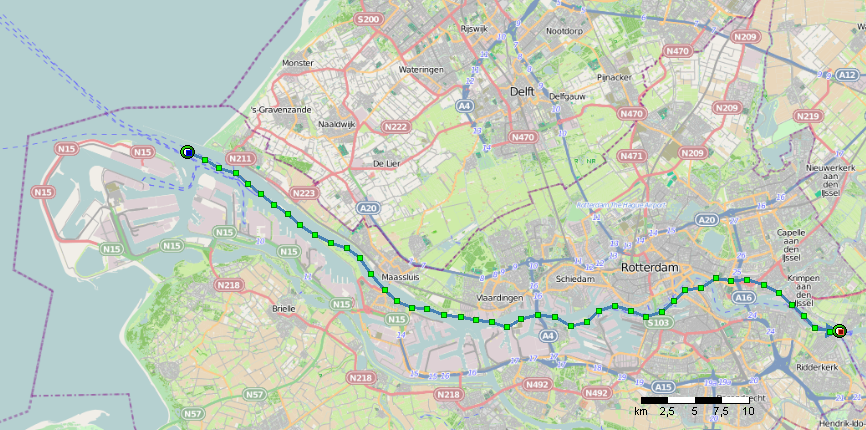
\includegraphics[width=\textwidth]{figures/chapter_overview/example_map.png}
	\caption{The central map view.}
	\label{fig:fig2.3}
\end{figure}
When working in the central map, for example on a network, it is possible to add, adjust or delete network components, which is described thoroughly in the dflow manual.

Results in charts windows (\Fref{fig:chartwindow}) are presented by combining a table view and a '$xy$'-plot. The user can visualize separate data points by selecting rows in the table view. The data that is presented in the chart window may also be exported to a *.csv file by clicking the \button{Csv export} button.
%
\begin{figure} [H]
	\centering
		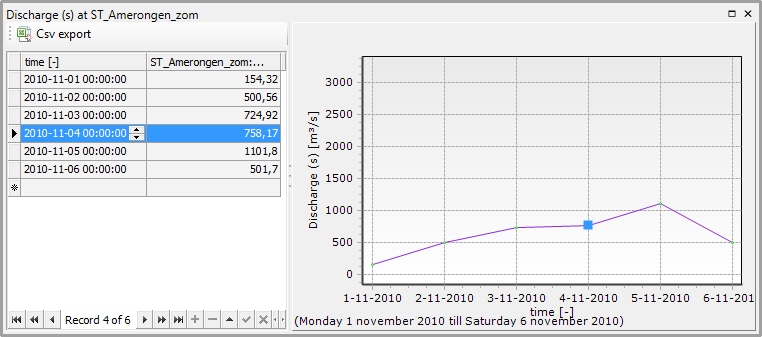
\includegraphics[width=\textwidth]{figures/chapter_overview/example_chart_window.png}
	\caption{The chart window view.}
	\label{fig:chartwindow}
\end{figure}

\subsection{Map}
\label{subsec:Map}
The \window{Map} window (\Fref{fig:fig2.4}) manages the active map. In this window layers within the active map can be shown, hidden or adjusted.
%
With the four icons in the top left of the window new \ext{shp}- or \ext{wms}-layers can be added, removed or exported. With the icons in the top right of the window, the window can be removed or hidden. The window can be retrieved by clicking on \button{Map} in \menu{View} ribbon.
%
\begin{figure} [H]
	\centering
		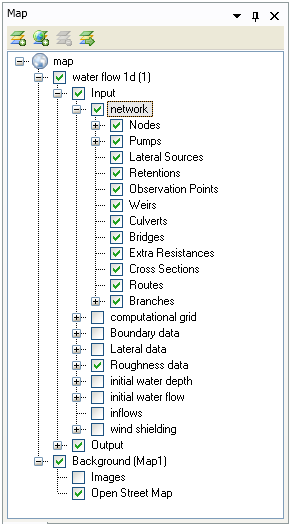
\includegraphics[width=0.5\textwidth]{figures/chapter_overview/view_map_window.png}
	\caption{The map window.}
	\label{fig:fig2.4}
\end{figure}

\subsection{Data}
\label{subsec:data}
The \window{Data} window (\Fref{fig:datawindow}) can be used to inspect the contents of available data items, when selected in the project window.
%
\begin{figure} [H]
	\centering
		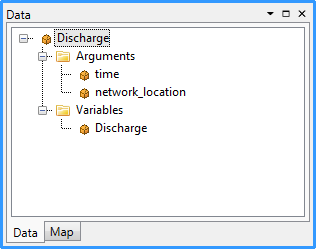
\includegraphics[width=0.5\textwidth]{figures/chapter_overview/view_data_window.png}
	\caption{The data window.}
	\label{fig:datawindow}
\end{figure}

\subsection{Chart}
\label{subsec:chart}
The \window{Chart} window (\Fref{fig:chartwindow}) can be used to stack/unstack chart series of the same type or to convert chart series to a certain type (area, line, point, or bar series), Furthermore, series can be selected or deselected within this window.
 
\begin{figure} [H]
	\centering
		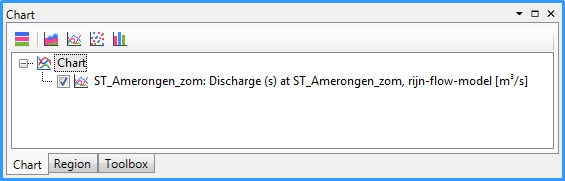
\includegraphics[width=0.5\textwidth]{figures/chapter_overview/view_chart_window.png}
	\caption{Example of the chart window.}
	\label{fig:chartwindow}
\end{figure}
%
\subsection{Properties}
\label{subsec:properties}
%
The \window{Properties} window shows properties for an active selection of the graphical user interface. When a model object is selected in the \window{Region} window it shows the properties of this object. Accordingly, the \window{Properties} window of an item selected in the \window{Project} shows data related to the selected item, for example the simulation time of a \dir{flow model} or a list with output parameters when clicking on the \dir{output} entry. \Fref{fig:fig2.6} shows an example for the properties of a flow model.

In the \window{Properties Window} data can also be edited. If the property grid is insufficient to display the information, for example in case of time series, an additional editor can be opened.
%
\begin{figure} [H]
	\centering
		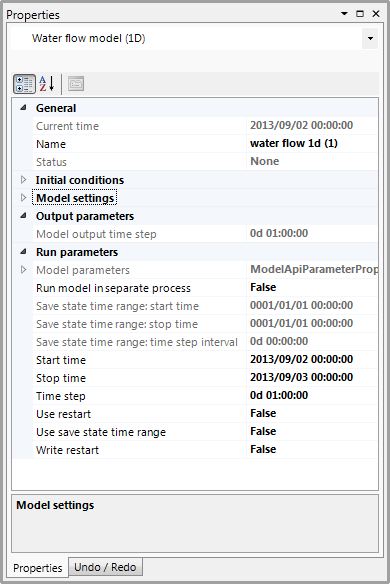
\includegraphics[width=0.5\textwidth]{figures/chapter_overview/view_properties_window.png}
	\caption{Example of a property grid in the properties window of a flow model.}
	\label{fig:fig2.6}
\end{figure}
%
\subsection{Messages}
\label{subsec:messages}
%
The \window{Messages} window (\Fref{fig:messageswindow}) is a logging window. Messages sent from models or different parts of the system are shown here. When a message is too large to fit within the \window{Messages} the user can open a single message (\Fref{fig:messagedetailwindow}) separately by right-mouse-clicking the message and selecting the 'Show details' option.
%
\begin{figure} [H]
	\centering
		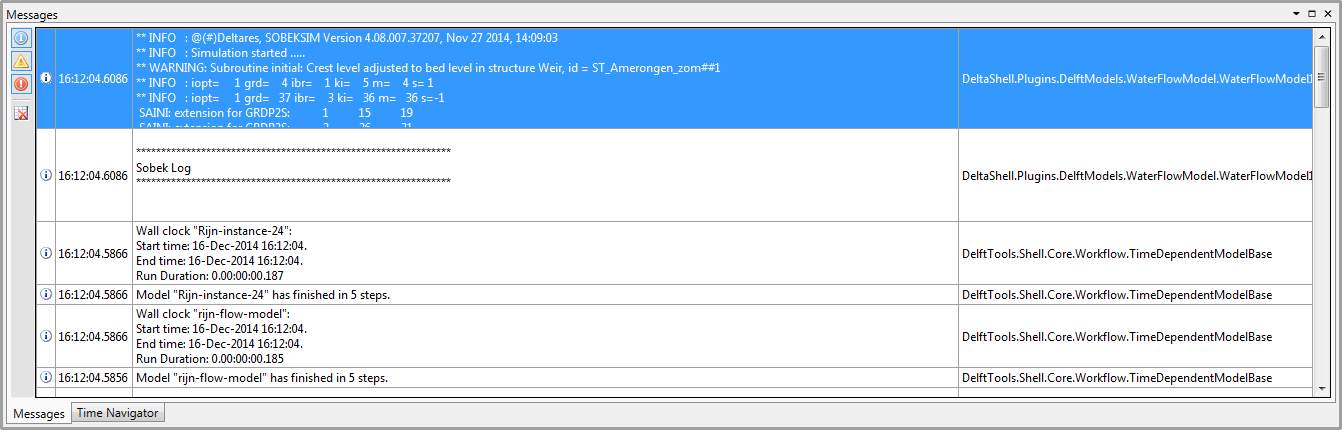
\includegraphics[width=\textwidth]{figures/chapter_overview/view_messages_window.png}
	\caption{The messages window.}
	\label{fig:messageswindow}
\end{figure}
%
\begin{figure} [H]
	\centering
		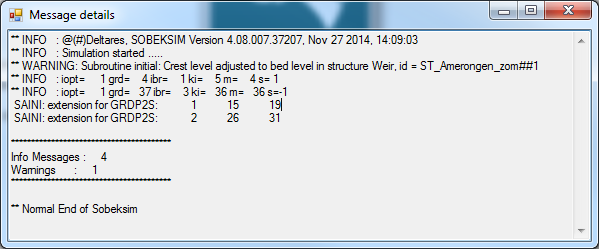
\includegraphics[width=0.5\textwidth]{figures/chapter_overview/view_messagedetails_window.png}
	\caption{The message detail window.}
	\label{fig:messagedetailwindow}
\end{figure} 

Within the \window{Messages} window the user may select the verbosity of the shown messages, ranging from 'Info messages' to 'Warning messages' to 'Error messages'. It is also possible to clear all messages by clicking 
\includegraphics[height=5mm]{figures/chapter_overview/icon_clear_all_messages}.

Furthermore, a run report is shown in the output in the \window{Project} for each model simulation. This run report contains all the messages (from DeltaShell and the model plug-ins) that occur during a simulation.

Finally, an application log is kept for each session of DeltaShell in the project database. In this log-file, which can be accessed through the \menu{File/Help} or \menu{Home} menus, all messages are stored.

% include section: Dockable views, which is also used in other separate User manuals
\svnid{$Id: section_dockableviews.tex 1 2015-08-30 15:39:28Z rodriqu_dd $}

\section{Dockable views}
\label{sec:dockableviews}
The  framework offers lots of freedom to customize dockable views, which are discussed in this section.
\subsection{Docking tabs separately}
\label{subsec:dockingtabs}
Within the  framework the user can dock the separate windows according to personal preferences. These preferences are then saved for future use of the framework. An example of such preferences is presented in \Fref{fig:exampledocking}, where windows have been docked on two screens.
%
\begin{figure} [H]
	\centering
		\includegraphics[width=\textwidth]{figures/chapter_overview/example_docking.png}
	\caption{Docking windows on two screens within the framework.}
	\label{fig:exampledocking}
\end{figure}

\subsection{Multiple tabs}
\label{subsec:multipletabs}
In case two windows are docked in one view, the underlying window (tab) can be brought to the front by simply selecting the tab, as is shown here.
%
\begin{figure} [H]
	\centering
		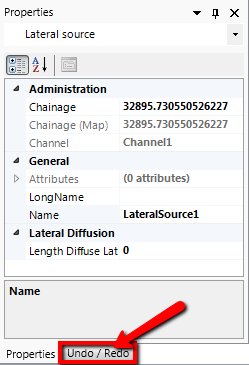
\includegraphics[width=0.5\textwidth]{figures/chapter_overview/example_docking_UndoRedo_1.png}
	\caption{Bringing the \window{Undo/Redo} window to the front}
\end{figure}
%
By dragging dockable windows with the left mouse button and dropping the window left, right, above or below another one the graphical user interface can be customized according to personal preferences. Here an example of the \window{Undo/Redo} window being docked above the \window{Properties} window.
%
\begin{figure} [H]
	\centering
		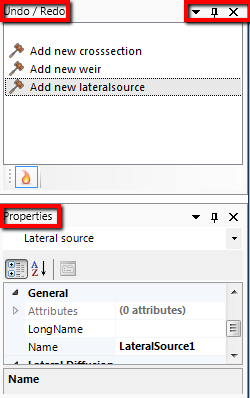
\includegraphics[width=0.5\textwidth]{figures/chapter_overview/example_docking_UndoRedo_2.png}
	\caption{Docking the \window{Undo/Redo} window.}
	\label{fig:docking}
\end{figure}
%
Additional features are the possibility to remove or (auto) hide the window (top right in \Fref{fig:docking}). In case of removal, the window can be retrieved by a mouse-click on \button{Undo/Redo} in the \menu{View} ribbon. Hiding the \window{Undo/Redo} window results in:
%
\begin{figure} [H]
	\centering
		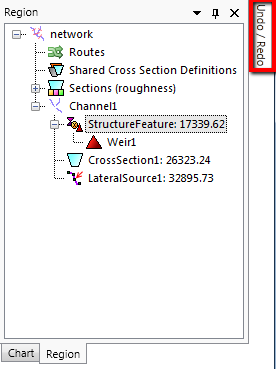
\includegraphics[width=0.5\textwidth]{figures/chapter_overview/example_autohide.png}
	\caption{Auto hide the \window{Undo / Redo} window}
\end{figure}

\section{Context menus}
\label{sec:contextmenus}
Depending on the active window, different context menus are present when right-mouse-clicking on items within this window. This section will treat these context menus per active window. 
%
\subsection{Project}
\label{subsec:project}
Within the \window{Project} window, a variety of levels and/or items with different context menus are present. These will be described here. 
\subsubsection{Project level}
\label{subsubsec:projectlevel}
The context menu of the project level within the project explorer is shown in \Fref{fig:contextmenuproject}. It contains the following choices:
%
\begin{figure} [H]
	\centering
		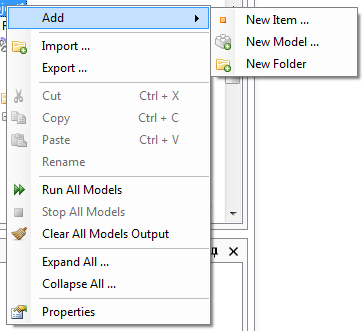
\includegraphics[width=0.5\textwidth]{figures/chapter_overview/context_menu_project.png}
	\caption{The context menu on the project level within the project explorer.}
	\label{fig:contextmenuproject}
\end{figure}
\begin{itemize}
	\item \button{Add} $\Rightarrow$ Option to add models and/or items to project (depending on installed model plug-ins)
	\item \button{Import \dots} $\Rightarrow$ Opens selection window for a variety of available importers (if present)
	\item \button{Export \dots} $\Rightarrow$ Opens selection window for a variety of available exporters (if present) 
	\item \button{Cut} $\Rightarrow$ Cuts current project for pasting elsewhere
	\item \button{Copy} $\Rightarrow$ Copies current project for pasting elsewhere
	\item \button{Paste} $\Rightarrow$ Pastes current project available on the clipboard
	\item \button{Rename} $\Rightarrow$ Rename the current project
	\item \button{Run All Models} $\Rightarrow$ Runs all models available in the project
	\item \button{Stop All Models} $\Rightarrow$ Stops running of all models currently running within the project
	\item \button{Clear All Models Output} $\Rightarrow$ Clears all model output of models available within the project
	\item \button{Expand All \dots} $\Rightarrow$ Expands all project items
	\item \button{Collapse All \dots} $\Rightarrow$ Collapses all project items
	\item \button{Properties} $\Rightarrow$ Switches to \window{Properties} window of active project
\end{itemize}
\subsubsection{Other level still to come}
\label{subsubsec:otherLevel1}
The context menu of \ldots 
%

\subsection{Main (Central Map window)}
\label{subsec:centralmap}
The \window{Main} or \window{Central Map} window may consist of multiple tabs \ldots

\subsubsection{Table editor}
\label{subsubsec:tableeditor}
The context menu of the table editors within the \window{Main} window as shown in \Fref{fig:contextmenutable} contains the following choices: 
%
\begin{figure} [H]
	\centering
		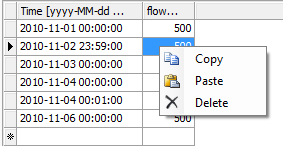
\includegraphics[width=0.4\textwidth]{figures/chapter_overview/context_menu_table.png}
	\caption{The context menu of the table editor.}
	\label{fig:contextmenutable}
\end{figure}
\begin{itemize}
	\item \button{Copy}
	\item \button{Paste}
	\item \button{Delete}
\end{itemize}
\subsubsection{Charts}
\label{subsubsec:charts}
The context menu of the charts within the \window{Main} window as shown in \Fref{fig:contextmenuchart} contains the following choice: 
%
\begin{figure} [H]
	\centering
		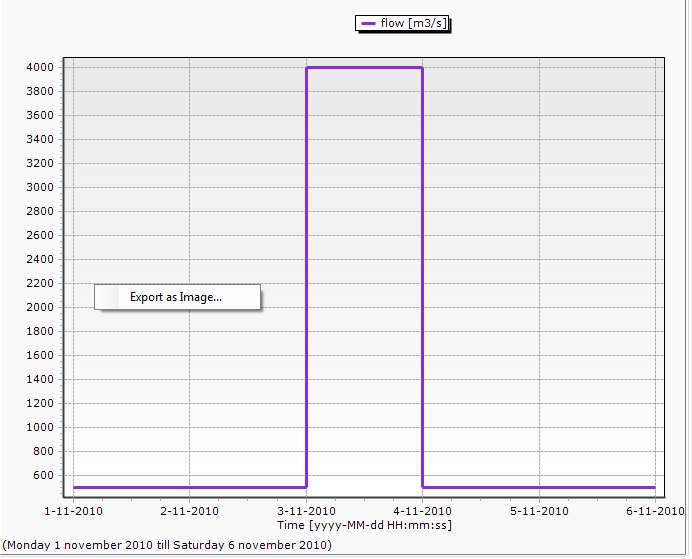
\includegraphics[width=0.8\textwidth]{figures/chapter_overview/context_menu_chart.png}
	\caption{The context menu of the chart view.}
	\label{fig:contextmenuchart}
\end{figure}
\begin{itemize}
	\item \button{Export as Image \dots}
\end{itemize}
\subsection{Map}
\label{subsec:map}
Beschrijving van Map panel.
%
\subsection{Messages}
\label{subsec:messages2}
The context menu for the \window{Messages} window as shown in \Fref{fig:contextmenumessages} contains the following choices: 
%
\begin{figure} [H]
	\centering
		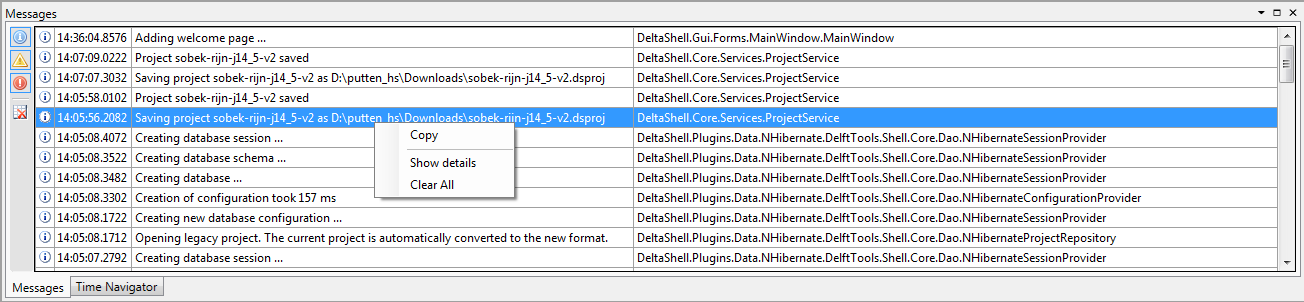
\includegraphics[width=\textwidth]{figures/chapter_overview/context_menu_messages.png}
	\caption{The context menu for the \window{Messages} window.}
	\label{fig:contextmenumessages}
\end{figure}
\begin{itemize}
	\item \button{Copy}
	\item \button{Show details} $\Rightarrow$ Open separate window with detailed message information
	\item \button{Clear all}
\end{itemize}

% include section: Ribbons and toolbars, which is also used in other separate User manuals
\svnid{$Id: section_ribbons.tex 1 2015-08-30 15:39:28Z rodriqu_dd $}

%-------------------------------------------------------------------------------
\section{Ribbons and toolbars}
\label{sec:ribbons}
The user can access the toolbars arranged in \menu{ribbons}. Failure mechanisms plug-ins can have their own specific \menu{ribbon}. The \menu{ribbon} may be auto collapsed by activating the \button{Collapse the Ribbon} button when right-mouse-clicking on the \menu{ribbon}.

%-------------------------------------------------------------------------------
\subsection{Ribbons (hot keys)}\label{subsec:gettingstarted_ribons}

WTI Ringtoets makes use of ribbons, just like Microsoft Office. You can use these ribbons for most of the operations. 
With the ribbons comes hot key functionality, providing shortcuts to perform operations.
If you press ``ALT'', you will see the letters and numbers to access the ribbons and the ribbon contents (i.e.\ operations). For example, ``ALT'' + ``H'' will lead you to the ``Home''-ribbon (\Fref{fig:ribbonhotkey}).

\textbf{\Note Implementation of the hot key functionality is still work in progress.}

\begin{figure}[H]
	\centering
	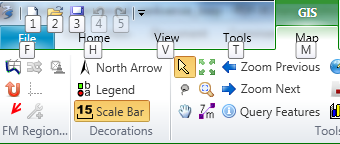
\includegraphics{figures/chapter_overview/ds_ribbon_hotkey.png}
	\caption{Perform operations using the hot keys} \label{fig:ribbonhotkey}
\end{figure}

%-------------------------------------------------------------------------------
\subsection{File}
\label{subsec:file}
The left-most \menu{ribbon} is the \menu{File} ribbon. It has menu-items comparable to most Microsoft applications. Furthermore, it offers users import and export functionality, as well as the \menu{Help} and \menu{Options} dialogs, as shown in \Fref{fig:ribbonfile} and \Fref{fig:dsoptions}.
%
\begin{figure} [H]
	\centering
		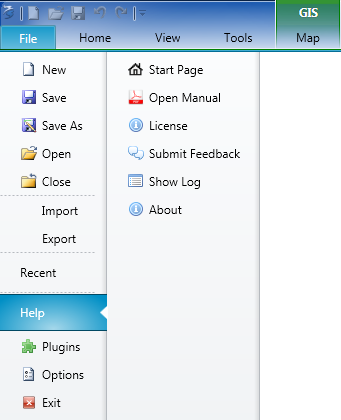
\includegraphics[width=0.6\textwidth]{figures/chapter_overview/ribbon_file.png}
	\caption{The \menu{File} ribbon.}
	\label{fig:ribbonfile}
\end{figure}
%
\begin{figure} [H]
	\centering
		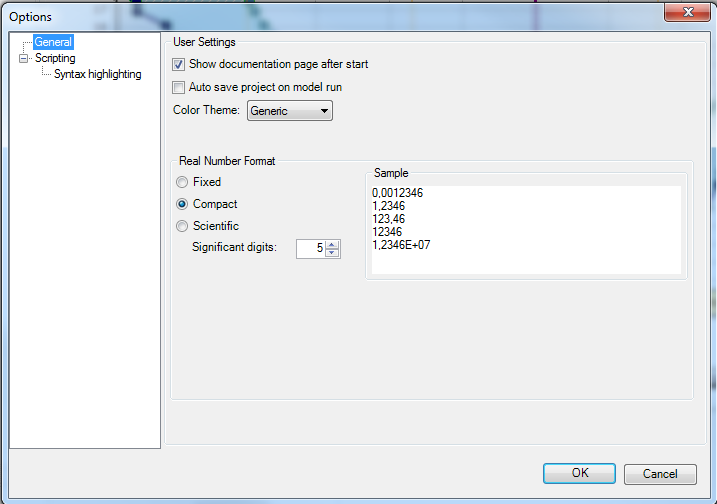
\includegraphics[width=\textwidth]{figures/chapter_overview/ds_options.png}
	\caption{The options dialog.}
	\label{fig:dsoptions}
\end{figure}

%-------------------------------------------------------------------------------
\subsection{Home}
\label{ssec:ribbonhome}
The second \menu{ribbon} is the \menu{Home} ribbon (\Fref{fig:ribbonhome}). It harbours some general features for clipboard actions, addition of items, running models, finding items within projects or views, and help functionality.
\begin{figure}[H]
	\centering
	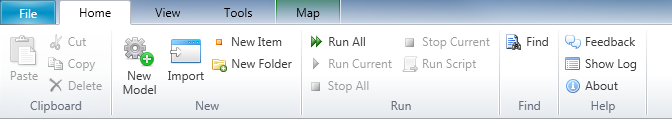
\includegraphics[width=1.0\textwidth]{figures/chapter_overview/ribbon_home.png}
	\caption{The \menu{Home} ribbon.}
	\label{fig:ribbonhome}
\end{figure}
%
%-------------------------------------------------------------------------------
\subsection{View}
\label{ssec:ribbonview}
The third \menu{ribbon} is the \menu{View} ribbon (\Fref{fig:ribbonview}). Here, the user can show or hide windows.
\begin{figure}[H]
	\centering
	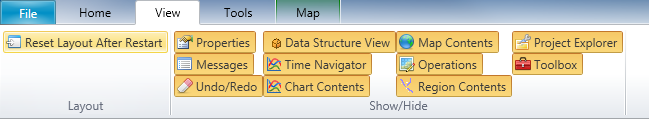
\includegraphics[width=0.5\textwidth]{figures/chapter_overview/ribbon_view.png}
	\caption{The \menu{View} ribbon.}
	\label{fig:ribbonview}
\end{figure}
%
%-------------------------------------------------------------------------------
\subsection{Tools}
\label{ssec:ribbontools}
The fourth \menu{ribbon} is the \menu{Tools} ribbon (\Fref{fig:ribbontools}). By default, it contains only the \menu{Open Case Analysis View} tool. Some model plug-ins offer the installation of extra tools that may be installed. These are documented within the user documentation of those model plug-ins. 
\begin{figure}[H]
	\centering
	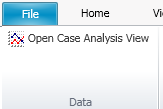
\includegraphics[width=0.2\textwidth]{figures/chapter_overview/ribbon_tools.png}
	\caption{The \menu{Tools} ribbon.}
	\label{fig:ribbontools}
\end{figure}
%
%-------------------------------------------------------------------------------
\subsection{Map}
\label{ssec:ribbonmap}
The last \menu{ribbon} is the \menu{Map} ribbon (\Fref{fig:ribbonmap}).
\begin{figure}[H]
	\centering
	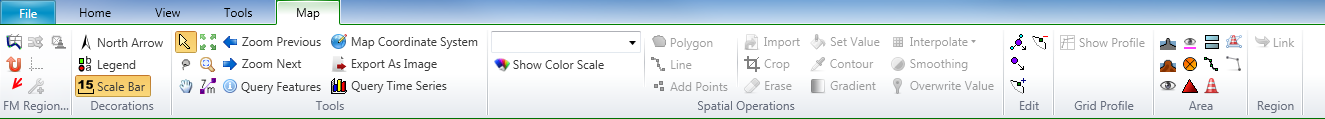
\includegraphics[width=1.0\textwidth]{figures/chapter_overview/ribbon_map.png}
	\caption{The \menu{Map} ribbon.}
	\label{fig:ribbonmap}
\end{figure}
%
This will be used heavily, while it harbours all \menu{Geospatial} functions, like:
\begin{itemize}
\item \menu{Decorations} for the map
\begin{itemize}
	\item North arrow
	\item Scale bar
	\item Legend
	\item ...
\end{itemize}
\item \menu{Tools} to customize the map view
\begin{itemize}
	\item Select a single item
	\item Select multiple items by drawing a curve
	\item Pan
	\item Zoom to Extents
	\item Zoom by drawing a rectangle
	\item Zoom to Measure distance
	\item ...
\end{itemize}
\item \menu{Edit} polygons, for example within a network, basin, or waterbody
\begin{itemize}
	\item Move geometry point(s)
	\item Add geometry point(s)
	\item Remove geometry point(s)
\end{itemize}
\item Creation of a model \menu{Network}, for example for \dflow
\begin{itemize}
	\item Add new Branch
	\item Split Branch
	\item Add Cross section
	\item Add Weir
	\item Add Pump
	\item ...
\end{itemize}
\end{itemize}
%
\Note The \menu{ribbons} adjust to the size of the application window. If, for what reason, the user wants to minimize the window, the ribbons might look like as shown in \Fref{fig:ribbonmapminimised}. Some of the \menu{ribbon} categories have been condensed into a single drop-down panel.
\begin{figure}[H]
	\centering
	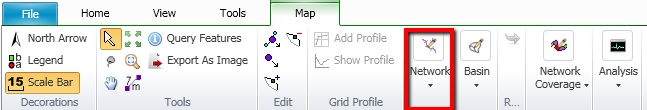
\includegraphics[width=0.8\textwidth]{figures/chapter_overview/ribbon_map_minimised.png}
	\caption{The ribbon with minimized categories.}
	\label{fig:ribbonmapminimised}		
\end{figure}
%
Still, all functions of the category can be activated as they will appear in the drop-down panel.
%
%-------------------------------------------------------------------------------
\subimport{chapters/}{ribbon_scripting}
%
%-------------------------------------------------------------------------------
\subsection{Quick access toolbar}
\label{ssec:Qaccestoolbar}
\Note The user can make frequently used functions available by a single mouse-click in the \menu{Quick Access Toolbar}, the top-most part of the application-window. Do this by right-mouse-clicking a ribbon item and selecting \menu{Add to Quick Access Toolbar}.
%
\begin{figure}[H]
	\centering
	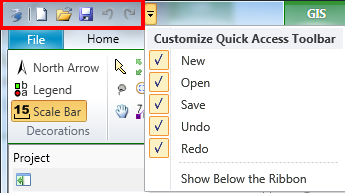
\includegraphics[width=0.6\textwidth]{figures/chapter_overview/quick_access_toolbar.png}
	\caption{The quick access toolbar.}
	\label{fig:qat}		
\end{figure}